\chapter{Mengenal Kecerdasan Buatan dan Scikit-Learn}

\section{Teori}
Praktek teori penunjang yang dikerjakan :
\begin{enumerate}
	\item Kecerdasan buatan atau Artificial Intelligence adalah suatu divisi ilmu komputer yang 
	mempelajari bagaimana membuat mesin (komputer) yang dapat bekerja sebaik yang dilakukan  manusia 
	dan bahkan dapat melakukan lebih baik dari apa yang dilakukan manusia.\\
	\par
	Menurut John McCarthy, 1956, kecerdasan buatan adalah mengidentifikasi dan memodelkan proses berpikir
	manusia dan merancang mesin untuk meniru perilaku manusia. Kecerdasan berarti memiliki pengetahuan 
	ditambah pengalaman, penalaran (bagaimana membuat keputusan dan bertindak), karakter yang baik.\\
	\par
	Orang pintar (smart) dalam memecahkan masalah karena orang memiliki pengetahuan dan pengalaman. Ilmu 
	itu didapat melalui belajar. Semakin banyak  pengetahuan yang Anda miliki, semakin baik pemecahan 
	masalah Anda. Namun memberikan pengetahuan saja tidak cukup, orang juga berhak untuk bernalar dan 
	menarik kesimpulan berdasarkan pengetahuan dan pengalaman yang dimilikinya.\\
	\par
	Tanpa penalaran yang baik, orang yang memiliki banyak pengalaman dan pengetahuan tidak akan mampu 
	menyelesaikan masalah dengan baik. Demikian pula dengan kemampuan penalaran yang sangat baik, namun 
	tanpa  pengetahuan dan pengalaman yang memadai, manusia juga tidak akan dapat menyelesaikan masalah 
	dengan baik.\\

	\item Definisi supervised learning, klasifikasi, regresi dan unsupervised learning. Data set, training set dan testing set
	\begin{itemize}
		\item Supervised Learning
		\par
		\textit{Supervised learning}
		adalah suatu pendekatan machine learning yang ditentukan berdasarkan penggunaan dataset, supervised learning menggunakan dataset berlabel atau labeled dataset. Supervised Learning digunakan untuk melakukan klasifikasi data atau memprediksi hasil secara akurat sesuai dengan output berdasarkan pola yang ada didalam data training dan berupa data yang memiliki label yang sudah ditentukan terlebih dahulu
		\item Unsupervised Learning
		\par
		\textit{Unsupervised Learning} adalah pendekatan machine learning yang digunakan untuk menganalisa dan juga mengelompokan kumpulan - kumpulan data yang tidak berlabel.
		\item Klasifikasi
		\par
		\textit{Klasifikasi} adalah sebuah proses menggunakan algoritma untuk secara akurat memasukan data kedalam kategori yang spesifik.
		\item Regresi
		\par
		\textit{Regresi} adalah sebuah proses menggunakan algoritma untuk memahami hubungan antara 2 variabel, yaitu variabel dependen dan variabel independen, Regresi dapat memprediksi nilai numerik variabel dependen berdasarkan variabel independen.
		\item Dataset
		\par
		\textit{Dataset} adalah suatu kumpulan data yang berisi informasi-informasi lama, dan dapat dikelola sehingga menjadi sebuah informasi baru.
		\item Training set
		\par
		\textit{Training set} adalah bagian dari dataset yang dilatih untuk kemudian digunakan untuk memprediksi sesuatu atau menjalankan fungsi dari algoritma.
		\item Testing set
		\par
		\textit{Testing set} adalah bagian dari dataset yang digunakan untuk melihat tingkat keakuratan dan performa dari algoritma.
	\end{itemize}

\end{enumerate}

\section{Instalasi}

\begin{enumerate}
\item Lakukan Installasi dalan CMD yang terdapat pada Anaconda dengan memasukan perintah "pip install -U scikit-learn".
\begin{figure}[!htbp]
	\centering
	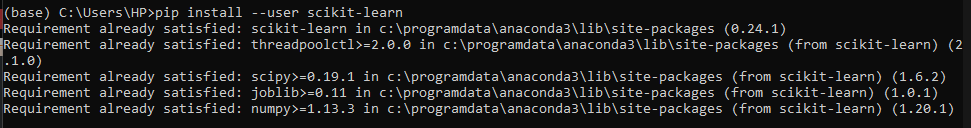
\includegraphics[scale=0.6]{figures/installscikitlearn.png}
\end{figure}
\item Untuk Modul Praktikum kita bisa melihatnya pada Link yang di sediakan. Dan sekarang kita akan melakukan import library datasets.
\begin{figure}[!htbp]
	\centering
	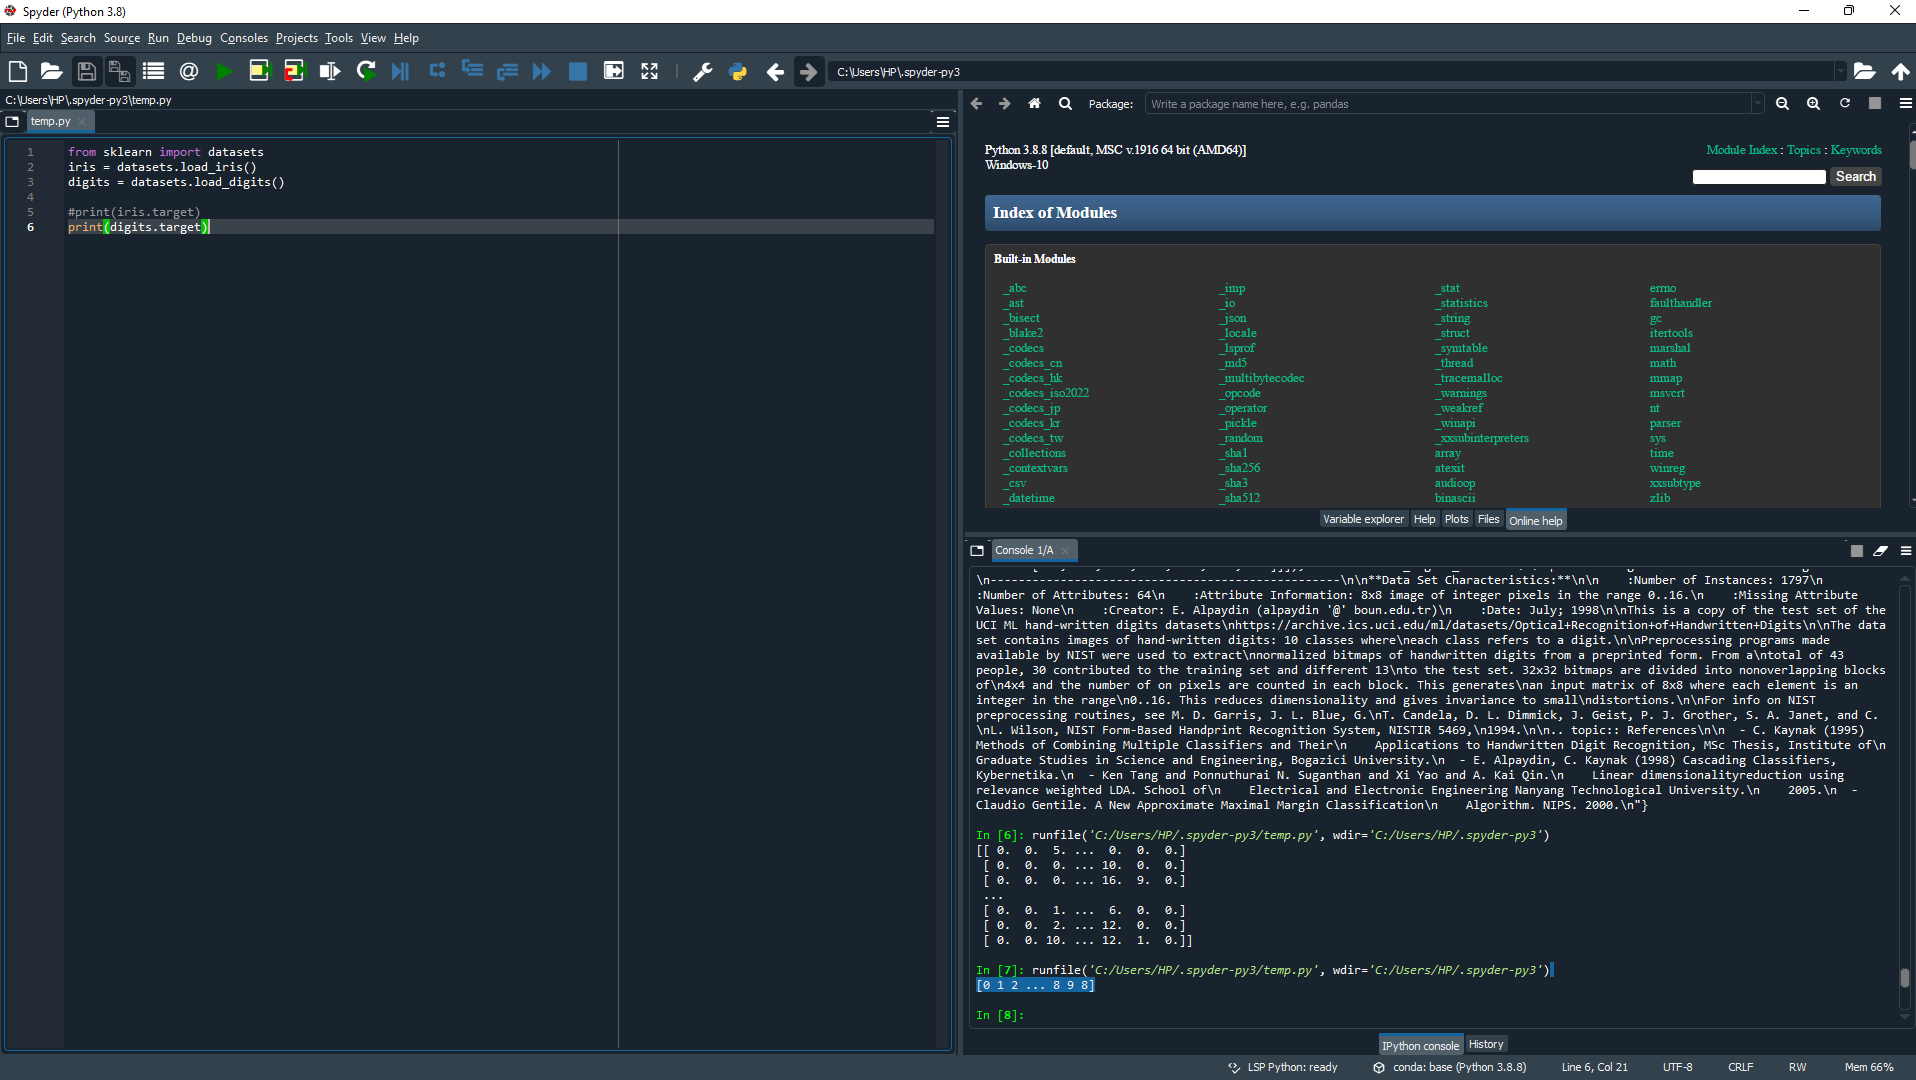
\includegraphics[scale=0.3]{figures/1.png}
\end{figure}
\newpage
\item Kita akan melakukan Modeling dengan metode SVM dengan method SVC() kemudian langsung mengklasifikasi hasil predict yang di lakukan dari model.
\begin{figure}[!htbp]
	\centering
	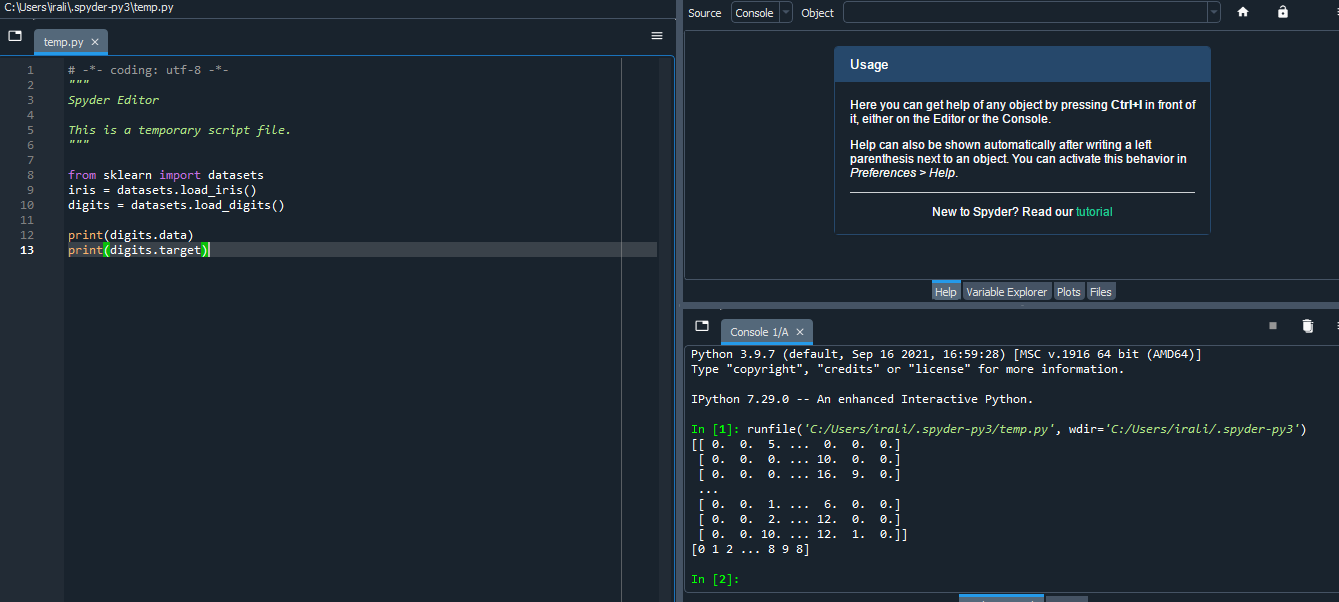
\includegraphics[scale=0.3]{figures/2.png}
\end{figure}
\item Kemudian kita akan melakukan Type Casting dengan menggunakan random number dengan library Numpy.Random.
\begin{figure}[!htbp]
	\centering
	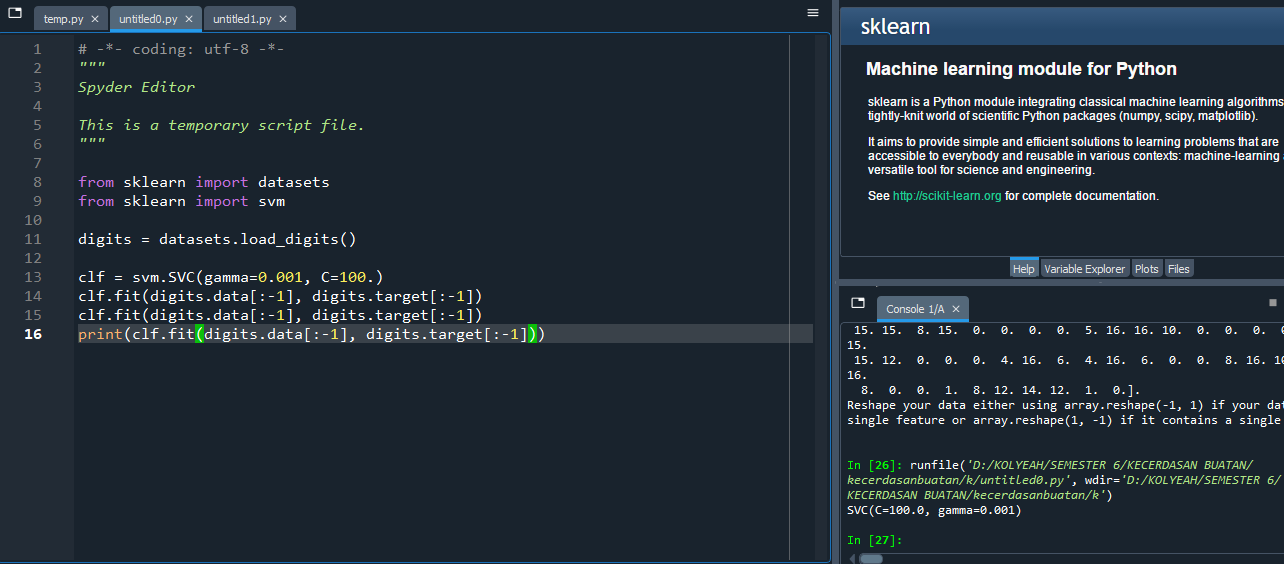
\includegraphics[scale=0.3]{figures/3.png}
\end{figure}
\newpage
\item Bagian untuk Refitting dan untuk mengupdate Paramters kita bisa menggunakan library load iris.
\begin{figure}[!htbp]
	\centering
	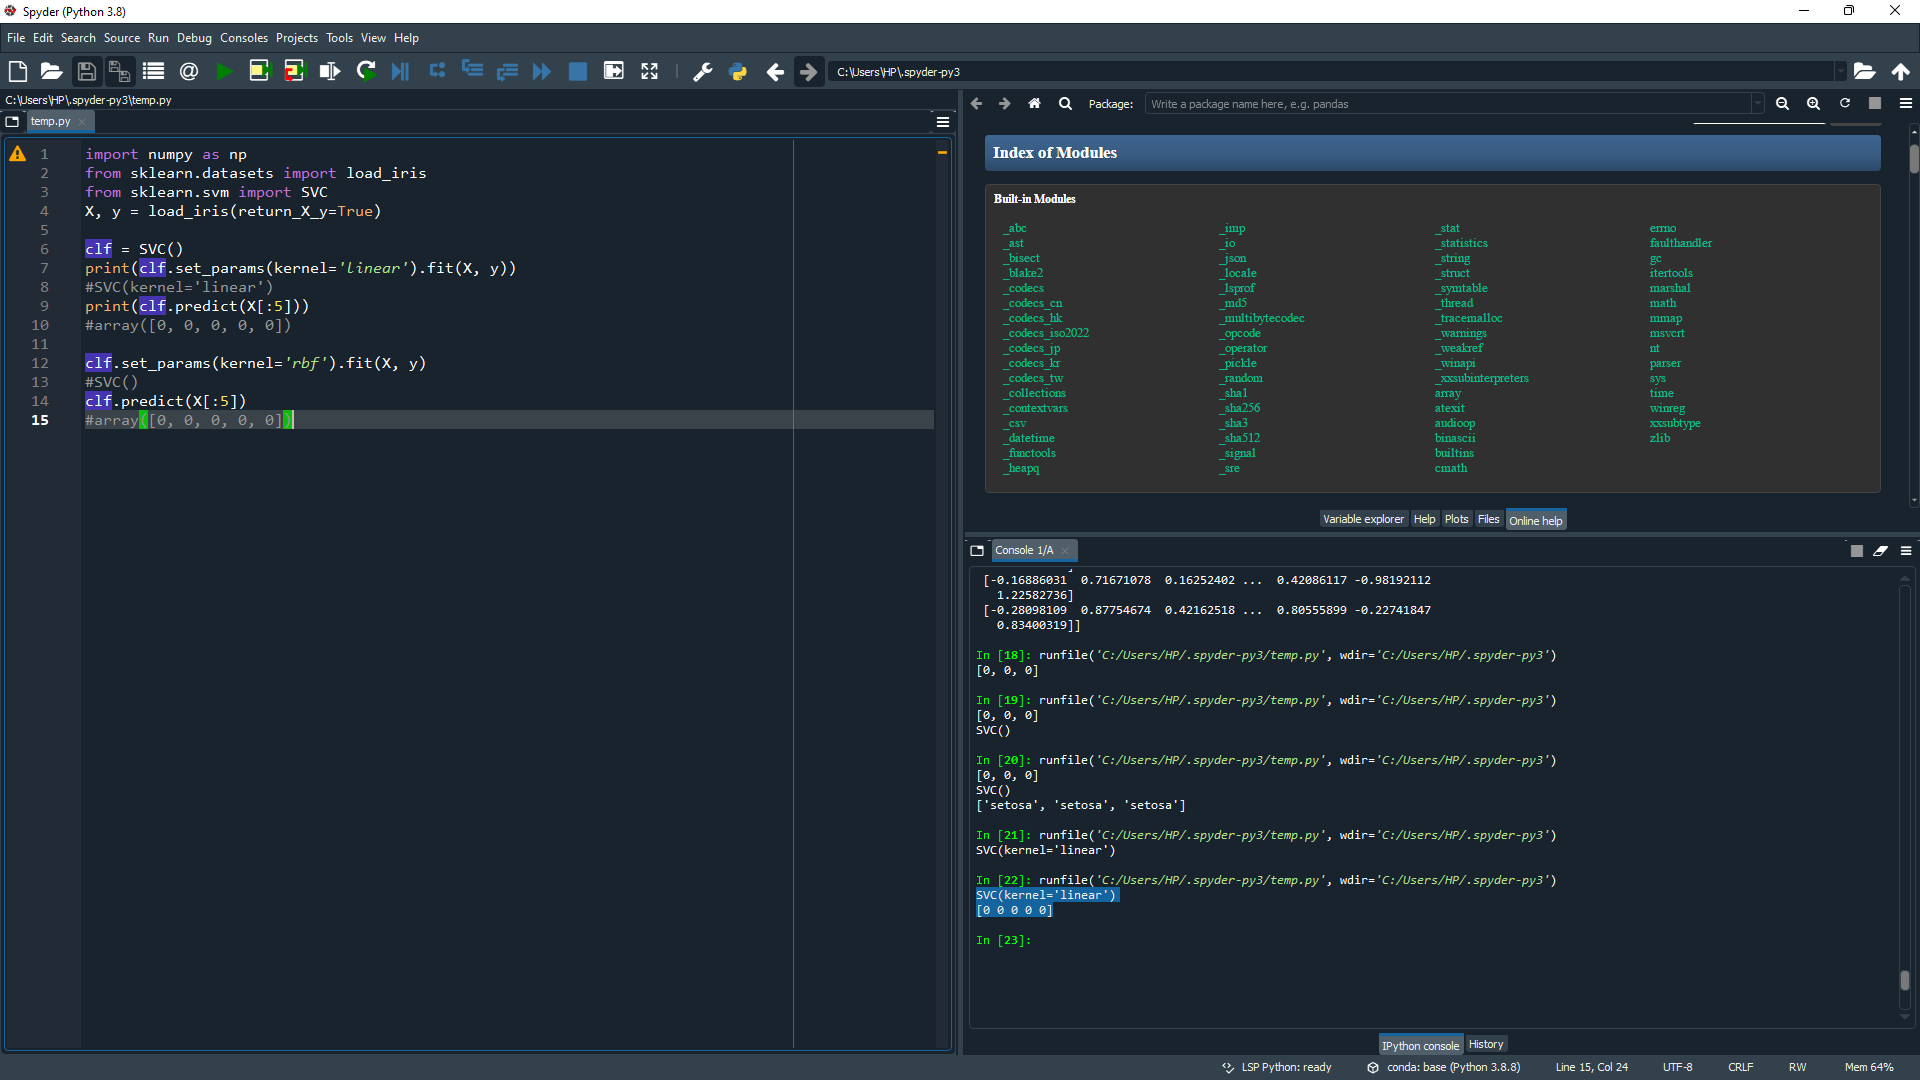
\includegraphics[scale=0.3]{figures/4.png}
\end{figure}
\item Untuk melakukan Refitting dan Update Paramters kita bisa menggunakan library OneVsRestClassifier dan LabelBinarizer.
\begin{figure}[!htbp]
	\centering
	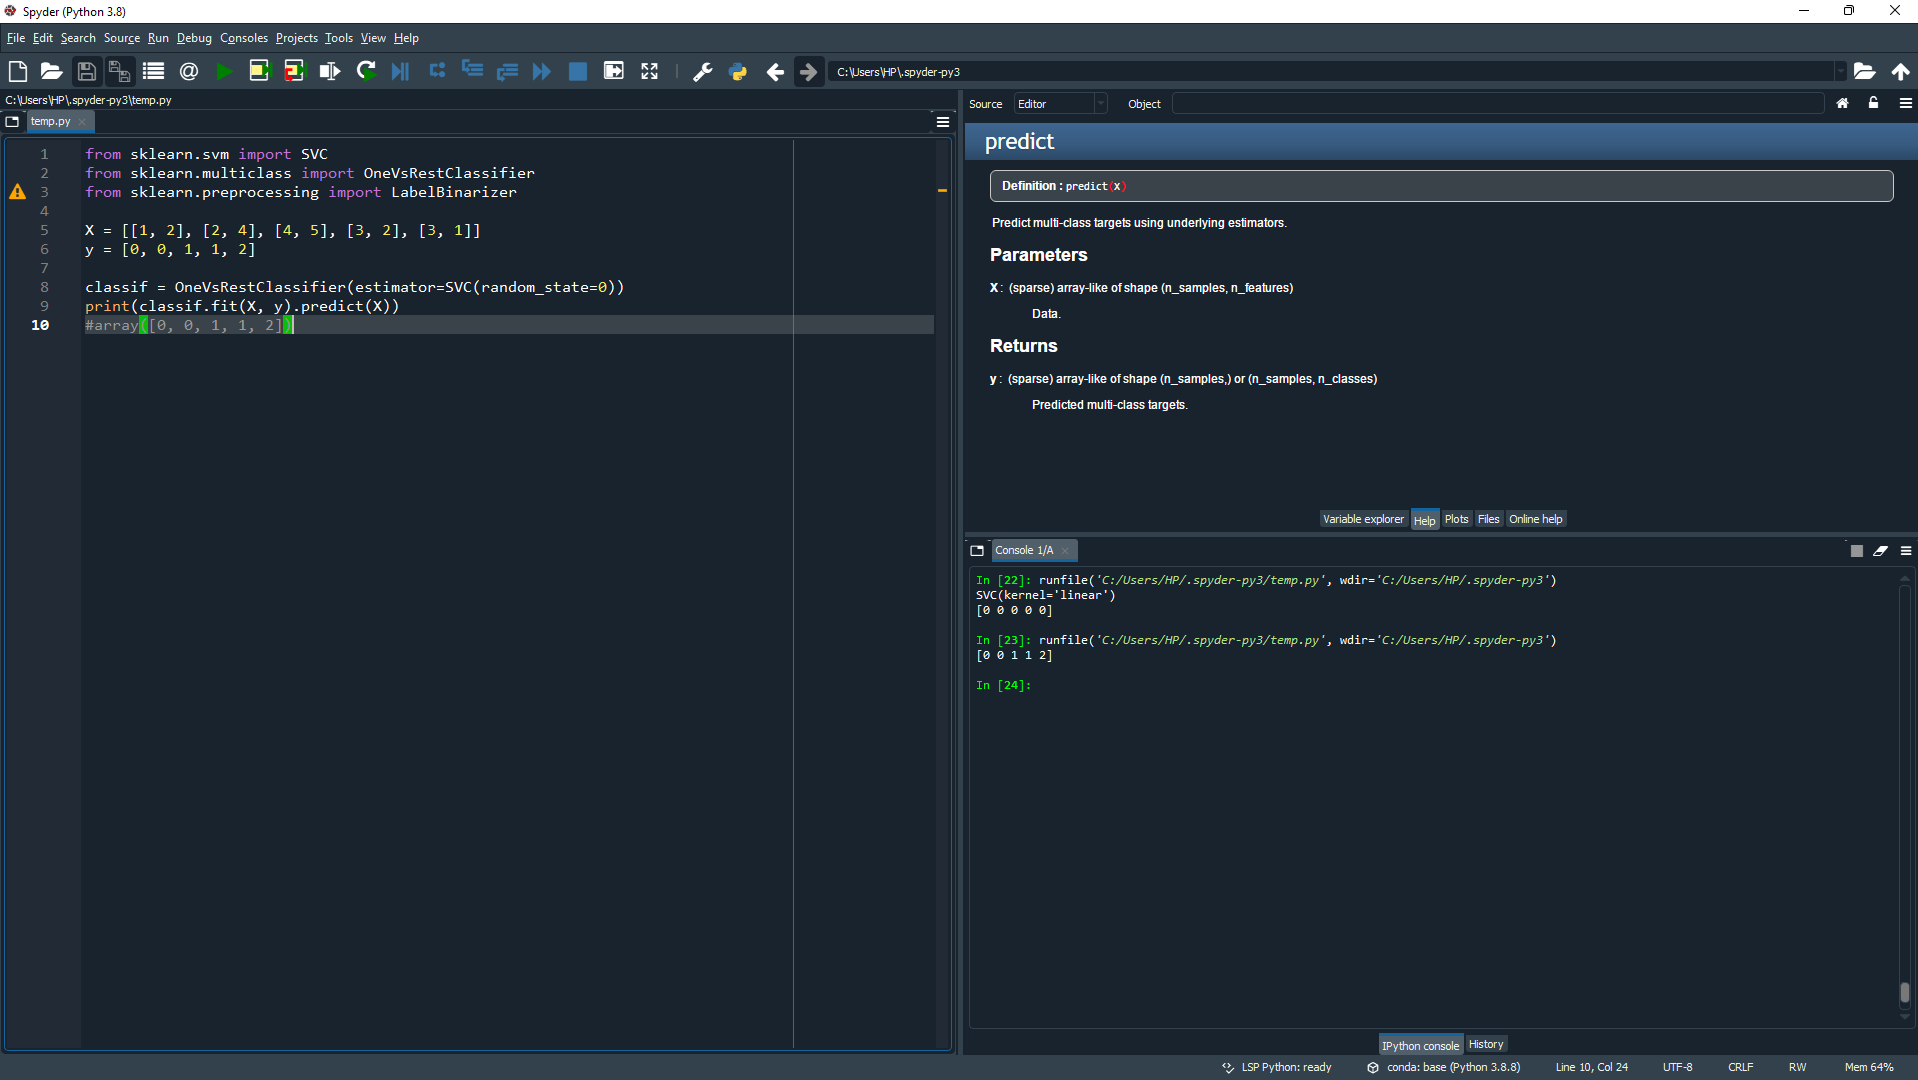
\includegraphics[scale=0.3]{figures/5.png}
\end{figure}
\newpage
\begin{figure}[!htbp]
	\centering
	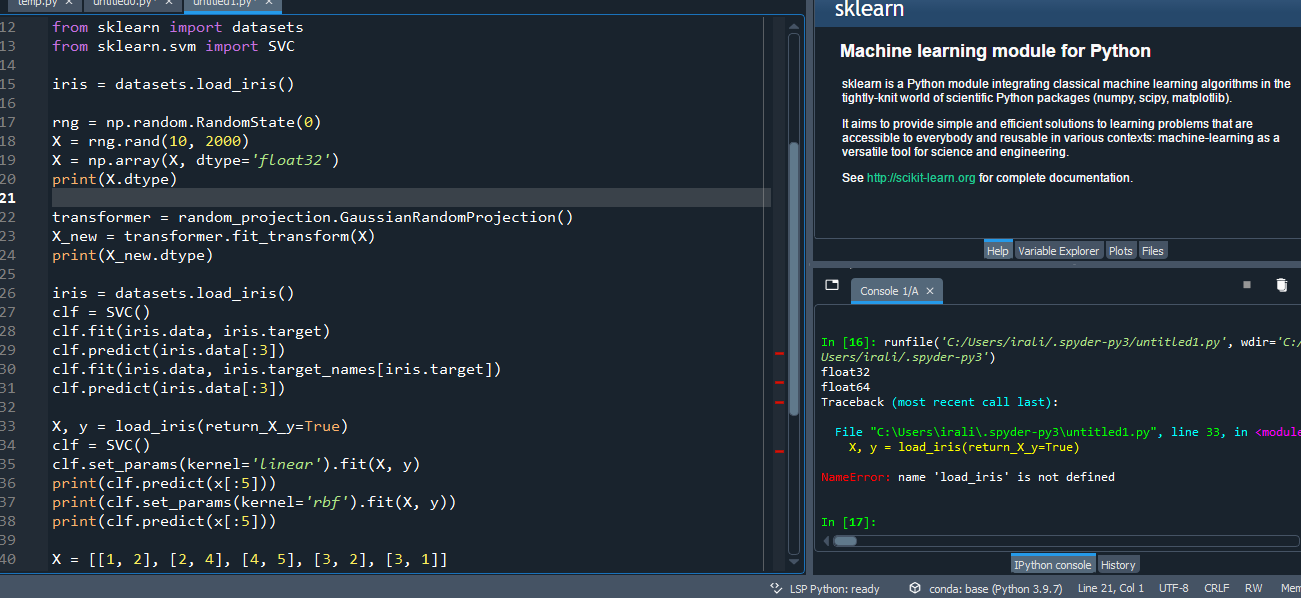
\includegraphics[scale=0.3]{figures/6.png}
\end{figure}

\end{enumerate}
\section{Penanganan Error}
Contoh - contoh error saat melakukan Praktikum :

\begin{enumerate}
\item Access Denied Install Scikit Learn.
\begin{figure}[!htbp]
	\centering
	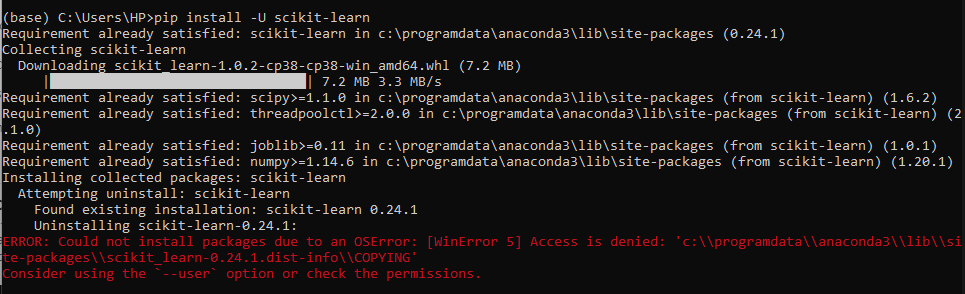
\includegraphics[scale=0.6]{figures/8.png}
\end{figure}
\item Undefinied Variabel or Modul.
\begin{figure}[!htbp]
	\centering
	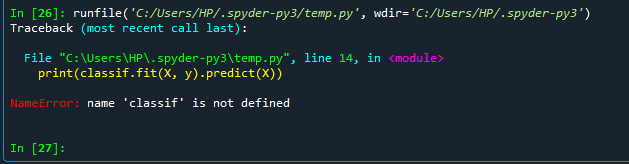
\includegraphics[scale=0.6]{figures/7.png}
\end{figure}
\newpage
\item Data not Support.
\begin{figure}[!htbp]
	\centering
	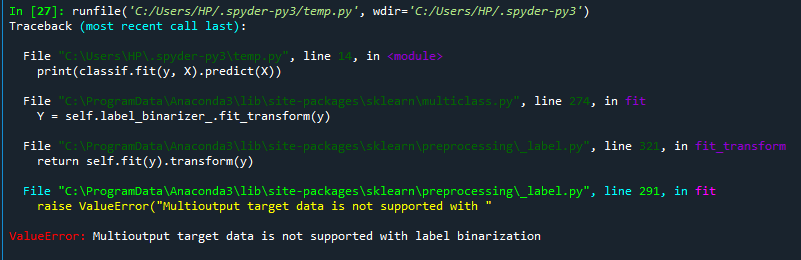
\includegraphics[scale=0.6]{figures/9.png}
\end{figure}
\item Expected array.
\begin{figure}[!htbp]
	\centering
	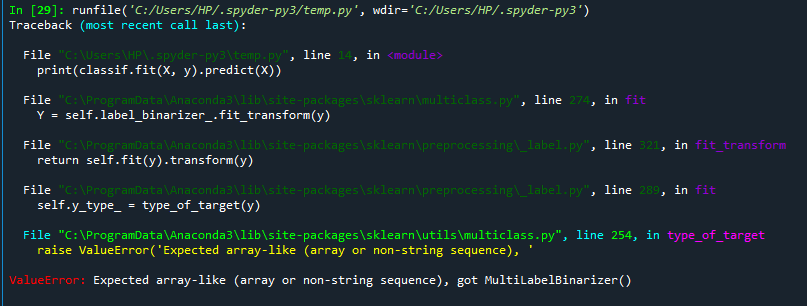
\includegraphics[scale=0.6]{figures/10.png}
\end{figure}

\item
Solusi dari masalah error tersebut :
\par
Access Denied Install Scikit Learn. Dengan memberitahukan komputer kalau yang lagi install adalah user dengan menambahkan --user pada saat penginstallan.
\par
Undefinied Variabel or Modul. Pastikan Variabel atau modul sudah di inisialisasikan atau belum.
\par
Data not Support. Data yang digunakan untuk train harus di pastikan apakah data train dengan parameter X dan Y dan jangan sampai terbalik penempatan parameternya.
\par
Expected array. Data yang digunakan untuk train harus di pastikan apakah data train sudah di Fit Transform atau belum.

\end{enumerate}
